\section{DevOps}

Im Folgenden werden alle Aspekte des DevOps-Prozesses beschrieben, 
die für die Entwicklung und den Betrieb der Anwendung relevant sind. 
Dies beinhaltet die Bereitstellung von Umgebungen, Rollen und Serviceaccounts, 
Pipelines und die Veröffentlichung neuer Features, die Einrichtung neuer Tenants, 
das Monitoring und das Load Testing.

\subsection{Umgebungen / Environments}

Für die Entwicklung und den Betrieb der Anwendung werden verschiedene Umgebungen (Environments) verwendet.
Für den Betrieb der Anwendung wird die \glqq{}Production\grqq{}-Umgebung verwendet, für 
die Entwicklung wird die \glqq{}Staging\grqq{}-Umgebung verwendet. 
Eine weitere \glqq{}Development\grqq{}-Umgebung wurde aufgrund der geringen Anzahl an Entwicklern 
nicht eingerichtet. Werden für die lokale Entwicklung Cloud-Dienste wie Firestore oder 
Storage Buckets benötigt, werden der Einfachheit halber diese aus der \glqq{}Staging\grqq{}-Umgebung 
verwendet.

Jede Umgebung wird in einem eigenen Projekt in der Google Cloud Platform betrieben.
So wird eine klare Trennung zwischen den Umgebungen gewährleistet.
Da beide Umgebungen über IAC (Infrastructure as Code) verwaltet werden,
sind die Umgebungen identisch und können außerdem schnell wiederhergestellt werden.

\subsubsection{Ressourcen pro Umgebung}

Tabelle \ref{tab:google-cloud-ressourcen} listet die Google Cloud Ressourcen pro Umgebung auf und
beschreibt kurz deren Funktion. Da die Umgebungen identisch sind, ist nur eine Tabelle notwendig.

\renewcommand{\arraystretch}{1.5}
{\rowcolors{2}{}{gray!20}
\begin{longtable}{l p{10cm}}
  \caption{Google Cloud Ressourcen pro Umgebung}
  \label{tab:google-cloud-ressourcen} \\
  \textbf{Ressource} & \textbf{Beschreibung} \\ [1ex]
  Kubernetes Cluster & Cluster, auf dem die Anwendung läuft. \\ [0.5ex]
  Storage Buckets  & Storage Buckets zur Speicherung von Defect Bildern, Defect Reports und anderen Dateien wie z.B. den Terraform State Files. \\ [0.5ex]
  Firestore & Firestore Datenbank zur Speicherung von Daten. \\ [0.5ex]
  Identity Platform & Identity Platform zur Verwaltung von Benutzern und Tenants \\ [0.5ex]
  Identity Federation & Identity Federation zur Authentifizierung von GitHub ohne Credentials. \\ [0.5ex]
  Cloud Run & Cloud Run für Services, die nicht im Kubernetes Cluster laufen. \\ [0.5ex]
  Artifact Registry & Ein Repository für Docker Images in der Artifact Registry \\ [0.5ex]
  DNS Zone & DNS Zone zur Verwaltung der Subdomains der einzelnen Tenants. \\ [0.5ex]
\end{longtable}}

\subsubsection{Tenant Isolation}

Die Isolation der Tenants im Kubernetes Cluster wird durch die Verwendung von Namespaces erreicht.
Es gibt einen Namespace für die \textit{free} Tenants und einen für die \textit{premium} Tenants.
Die Tenants in den \textit{free} bzw. \textit{premium} Namespaces teilen sich die dem Namespace zugewiesenen Ressourcen.
Enterprise Tenants erhalten einen eigenen Namespace. 
Die darin enthaltenen Ressourcen sind nur für diesen Tenant verfügbar.

Die Isolation der Tenants in der Google Cloud Platform wird durch die Verwendung von 
separaten Buckets und Firestore Datenbanken erreicht. Die Ressourcen werden dabei 
analog zu den Kubernetes Namespaces aufgeteilt. Die \textit{free} und \textit{premium} Tenants
teilen sich die Ressourcen wie Buckets und Firestore Datenbanken. Die Enterprise Tenants
erhalten eigene Ressourcen.

Für die Isolation innerhalb der geteilten Ressourcen, werden in den Buckets Unterordner und in 
den Firestore Datenbanken separate Collections für die Tenants angelegt.

\subsection{Roles and Role Mapping}

Da das Team aus nur drei Mitgliedern besteht, wurde auf eine detaillierte Aufteilung der Rollen unter
den Teammitgliedern verzichtet. Jedes Teammitglied hat Zugriff auf alle Ressourcen in dem jeweiligen Projekt.
Dafür wurde jedem Teammitglied die Rolle \textit{roles/owner} zugewiesen.

\subsubsection{Dienstkonten}

Um die einzelnen Services der Park Anwendung zu authentifizieren, wurde pro Service ein Dienstkonto erstellt.
Genauer wurde pro Service pro Namespace ein Dienstkonto angelegt weil ein Service aus dem \textit{free}
Namespace nicht auf die Ressourcen eines Services aus dem \textit{premium} Namespace zugreifen darf.

Um keine Credentials in den Services speichern zu müssen, 
wurde die \glqq{}Workload Identity Federation for GKE\grqq{}\footnote{https://cloud.google.com/kubernetes-engine/docs/concepts/workload-identity} verwendet.
Diese muss bei der Erstellung des Clusters aktiviert werden und läuft auf den Nodes des Clusters. 
Die Workload Identity Federation unterscheidet zwischen Dienstkonten 
der Google Cloud Platform und Dienstkonten des Kubernetes Clusters.

\begin{itemize}
  \item \textbf{Kubernetes-Dienstkonten} sind Kubernetes-Ressourcen, die eine Identität für Prozesse bereitstellen, 
  die in Ihren GKE-Pods ausgeführt werden.
  \item \textbf{IAM-Dienstkonten} sind Google Cloud-Ressourcen, 
  mit denen Anwendungen autorisierte Aufrufe an Google Cloud APIs ausführen können.
\end{itemize}

Die Workload Identity Federation ermöglicht es, dass ein Kubernetes-Dienstkonto auf ein IAM-Dienstkonto gemappt wird.
Damit das Mapping funktioniert, muss das Kubernetes-Dienstkonto in der Annotation 
\textit{iam.gke.io/gcp-service-account} die E-Mail-Adresse des IAM-Dienstkontos enthalten.
\footnote{https://cloud.google.com/kubernetes-engine/docs/how-to/workload-identity\#kubernetes-sa-to-iam}


Um den Zugriff auf die Google Cloud Ressourcen aus GitHub Actions zu ermöglichen,
wurde pro Projekt ein weiteres Dienstkonto erstellt. Dieses Dienstkonto hat nur die minimalen Rechte,
die für die Ausführung der GitHub Actions notwendig sind. Durch die \glqq{}Workload Identity Federation\grqq{}
(das ist eine andere Workload Identity Federation als die für GKE) müssen keine Credentials
in den GitHub Secrets gespeichert werden.\footnote{https://cloud.google.com/blog/products/identity-security/enabling-keyless-authentication-from-github-actions?hl=en}

\subsection{Pipelines and Release of new Features}

Für die Bereitstellung von neuen Features und Bugfixes wird ein CI/CD-Prozess verwendet.
Die CI/CD-Pipeline wird mit GitHub Actions realisiert.
Die gesamte Pipeline ist in mehrere Actions unterteilt, wobei die eine Action bei Pull-Requests ausgeführt wird,
die andere bei einem Push auf den \textit{dev}- oder \textit{main}-Branch.

\subsubsection*{Pipeline für Pull-Requests auf \textit{dev} und \textit{main}}

Die Pipeline für Pull-Requests besteht aus den folgenden Jobs:
\begin{itemize}
  \item \textbf{Build}: Die Docker Images aller Services werden gebaut und auf eventuelle Fehler überprüft.
  \item \textbf{Test}: Die Unittests der Services werden ausgeführt.
  \item \textbf{Plan Terraform for the Infrastructure}: Die Änderungen an der Infrastruktur werden geplant.
  \item \textbf{Plan Terraform for the Application}: Die Änderungen an der Anwendung werden geplant.
\end{itemize}

Je nachdem, ob es sich um einen Push auf den \textit{dev}- oder \textit{main}-Branch handelt, wird die Pipeline
für die \textit{staging}- oder \textit{production}-Umgebung ausgeführt. 
Abbildung \ref{fig:pr-pipeline} zeigt die Pipeline für Pull-Requests.

\begin{figure}[ht]
  \centering
  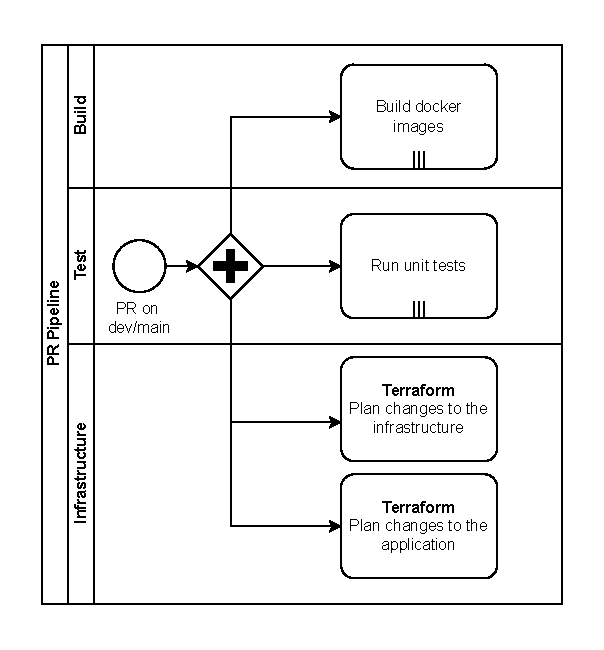
\includegraphics[width=0.6\textwidth]{resources/pr-pipeline.pdf}
  \caption{PR Pipeline}
  \label{fig:pr-pipeline}
\end{figure}


\subsubsection*{Pipeline für Push auf \textit{dev} und \textit{main}}

Die Pipeline für einen Push auf den \textit{dev}- oder \textit{main}-Branch ist für das 
Deployment der Änderungen in der Infrastruktur und der Anwendung zuständig.
Die Pipeline besteht aus den folgenden Jobs:

\begin{itemize}
  \item \textbf{Apply Terraform for the Infrastructure}: Die Änderungen an der Infrastruktur werden angewendet.
  \item \textbf{Build and Push Images}: Die Docker Images aller Services werden gebaut und in die Artifact Registry hochgeladen.
  \item \textbf{Package Cloud Functions}: Die Cloud-Functions werden in ein Zip-Archiv gepackt.
  \item \textbf{Apply Terraform for the Application}: Die Änderungen an der Anwendung werden angewendet. Das beinhaltet das Deployment der Docker Images und der Cloud-Functions.
  \item \textbf{Deploy Cloud Run}: Cloud-Run-Services, die nicht im Kubernetes Cluster laufen, werden deployed.
  \item \textbf{Update deployment.json}: Deployment-Informationen wie der Tag der Images werden in einer JSON-Datei in einem Bucket für spätere Pipelines gespeichert.
\end{itemize}

Da die Park Anwendung Multi-Tenant-fähig ist, müssen die Tenants auch in den Pipelines berücksichtigt werden.
Viele Ressourcen wie Buckets, Firestore Datenbanken und DNS-Zonen müssen pro Enterprise Tenant erstellt werden.
Um herauszufinden, ob Ressourcen erstellt, aktualisiert oder gelöscht werden müssen, wird eine JSON-Datei 
aus einem Bucket geladen. Diese Datei enthält die Konfiguration der Enterprise Tenants.

Je nachdem, ob es sich um einen Push auf den \textit{dev}- oder \textit{main}-Branch handelt, wird die Pipeline
für die \textit{staging}- oder \textit{production}-Umgebung ausgeführt.
Abbildung \ref{fig:cd-pipeline} zeigt die Pipeline für einen Push auf den \textit{dev}- oder \textit{main}-Branch.

\begin{figure}[ht]
  \centering
  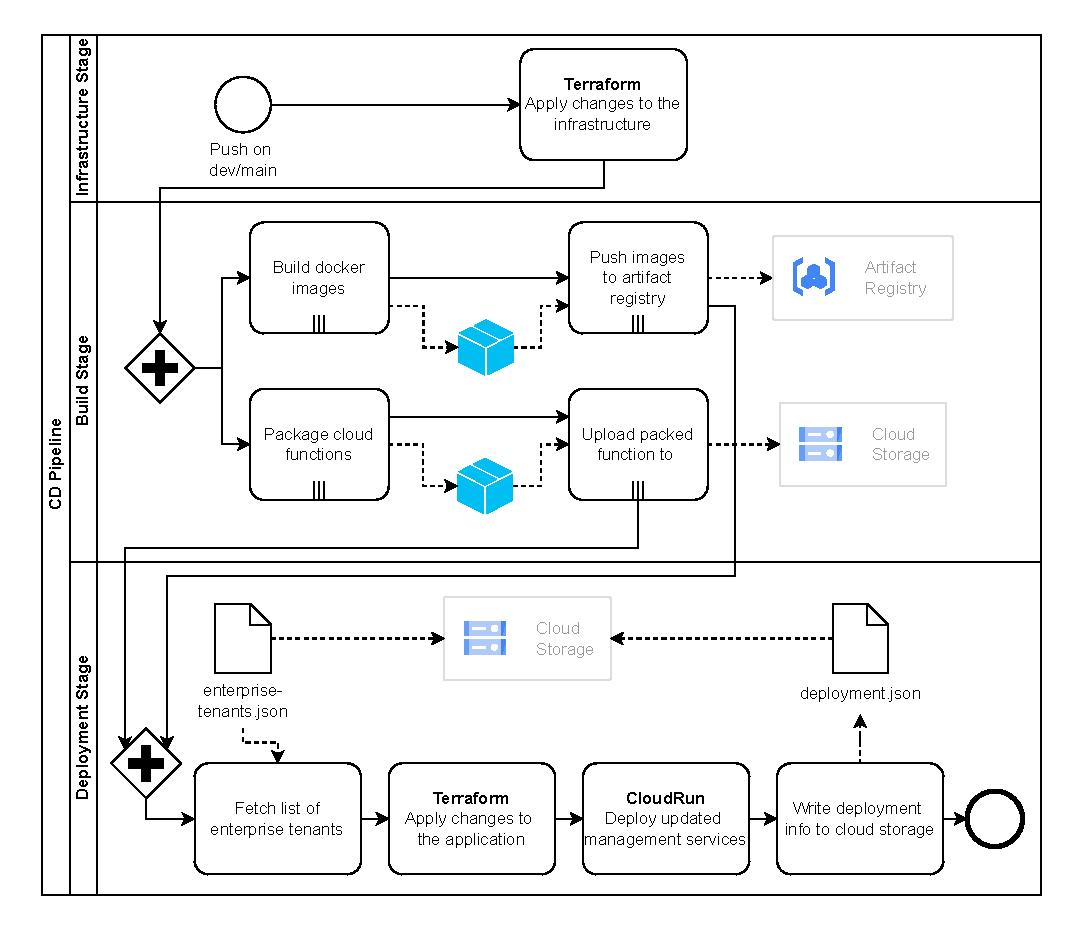
\includegraphics[width=\textwidth]{resources/cd-pipeline.pdf}
  \caption{CD Pipeline}
  \label{fig:cd-pipeline}
\end{figure}



\subsection{New Tenants}
\subsection{Monitoring}
\subsection{Load Testing}